\documentclass[]{rsos}%%%%where rsos is the template name

%%%% *** Do not adjust lengths that control margins, column widths, etc. ***


%%%%%%%%%%% Defining Enunciations  %%%%%%%%%%%
\newtheorem{theorem}{\bf Theorem}[section]
\newtheorem{condition}{\bf Condition}[section]
\newtheorem{corollary}{\bf Corollary}[section]
%%%%%%%%%%%%%%%%%%%%%%%%%%%%%%%%%%%%%%%%%%%%%%%



\begin{document}

%%%% Article title to be placed here
%\title{Zebrafish survival depends on escaping predators from a distance}
%\title{Enhanced performance in sensing, and not locomotion, improves survival in zebrafish prey}
%\title{Enhanced locomotor performance does not improve survival in zebrafish prey}
\title{A faster escape does not enhance survival in zebrafish larvae}


\author{%%%% Author details
Arjun Nair, Christy Nguyen, and Matthew J. McHenry}

%%%%%%%%% Insert author address here
\address{Department of Ecology and Evolutionary Biology\\
University of California, Irvine\\
321 Steinhaus Hall\\
Irvine, CA 92697}

%%%% Subject entries to be placed here %%%%
\subject{Animal behavior, biomechanics}

%%%% Keyword entries to be placed here %%%%
\keywords{pursuit-evasion model, locomotion, predation, sensing, strategy}

%%%% Insert corresponding author and its email address}
\corres{Matthew J. McHenry\\
\email{mmchenry@uci.edu}}



%%%%%%%%%%%%%%% End of first page %%%%%%%%%%%%%%%%%%%%%

\maketitle

%%%%%%%%%% Insert the texts which can accomdate on firstpage in the tag "fmtext" %%%%%

%\begin{fmtext}


\linespread{1.3}\selectfont %Doublespacing


\section*{Abstract}
An escape response is a rapid maneuver used by prey to evade predators. 
Performing this maneuver at greater speed, in a favorable direction, or from a longer distance have been hypothesized to enhance the survival of prey, but these ideas are difficult to test experimentally.
We examined how prey survival depends escape kinematics through a novel combination of experimentation and mathematical modeling. 
This approach focused on zebrafish (\textit{Danio rerio}) larvae under predation by adults and juveniles of the same species.
High-speed 3D kinematics were used to track the body position of prey and predator and to determine the probability of behavioral actions by both fish.
These measurements provided the basis for an agent-based probabilistic model that simulated the trajectories of the animals.
Predictions of survivorship by this model were found by Monte-Carlo simulations to agree with our observations and we examined how these predictions varied by changing individual model parameters.
Contrary to expectation, we found that survival may not be improved by increasing the speed or altering the direction of the escape.
Rather, zebrafish larvae operate with sufficiently high locomotor performance due to the relatively slow approach and limited range of suction feeding by the fish predators.
We did find that survival was enhanced when prey responded from a greater distance.
This is an ability that depends on the capacity of the visual and lateral line systems to detect a looming threat.
Therefore, performance in sensing, and not locomotion, is decisive for improving the survival of larval fish prey.
These results offer a framework for understanding the evolution of predator-prey strategy that may inform prey survival in a broad diversity of animals.


\section{Introduction}
An escape response allows prey to evade predators with rapid locomotion \cite{Bullock:1984gd}.
Because of its potential to directly affect survivorship, natural selection may favor animals that can execute an escape response with high locomotor performance.
Indeed, the physiology and mechanics of locomotion features many traits that appear to be adaptations for a rapid response and fast motion.
Escape responses are controlled by large-diameter command neurons (e.g. the giant axon of squid \cite{YOUNG:1938vi}), which often recruit specialized muscles (e.g. the axial musculature of fish \cite{Eaton:1975ux}), which may animate an appendage that is dedicated to escape behavior (e.g. the uropods of crayfish \cite{Johnson:1926cl}).
Prey may direct this escape in an optimal direction \cite{Weihs:1984tb}, or may alternatively benefit from moving randomly so as not to be predictable \cite{Humphries:1970hy,Howland:1974ud}.
However, it does not necessarily follow that any enhancement in speed or variation in heading will have a positive effect on a prey's survival.
Fish predators commonly approach their prey at a relatively slow speed \cite{Webb:1984jz,Higham:2007go} and this could permit escape by a prey operating below its maximal capacity. 
The aim of the present study was to test whether improvements in kinematics related to locomotor performance and sensing affect prey survival by examining predator-prey interactions in zebrafish (\textit{Danio rerio}, Hamilton 1922).

We addressed this aim with a novel approach that combines experimentation with mathematical modeling.
Our methodology was developed to meet the challenges to understanding the coupled dynamics of predators and prey.
Due to the sensing of both animals, the actions of the prey may (or may not) be a response to the predator, which may (or may not) be a response to prior motion by the prey. 
Regression analysis is generally insensitive to such interdependency, yet may succeed in resolving dominant features of successful prey \cite{Walker:2005vn} or predators \cite{Wainwright:2001ufa}.
It has additionally been helpful to study behavioral responses to an artificial predator or prey that is experimentally controlled and therefore not coupled to the actions of the animal \cite{Gabbiani:1999wz,Stewart:2014cma,Heuch:2007kk,Wainwright:2001ufa,Shifferman:2004fs}.
An alternative approach has attempted to formulate a behavioral algorithm of one animal by considering their responses to the measured kinematics of the other \cite{Ghose:2006dk}. 
Our recent approach similarly included measurements of predator-prey kinematics, but these were used as a basis for an agent-based probabilistic model that calculated the trajectories of both animals from a series of behavioral actions. 
A series of simulations by this model allowed for a predictive consideration of the effects of differences in behavior on prey survival.

Zebrafish provide an excellent experimental subject for studying the mechanisms of predator-prey interactions. 
The larval stage of this species serves as a model for the neurophysiological \cite{Bianco:2015gm,Bagnall:2014iu,Huang:2013vj} and biomechanical \cite{Muller:2004hp,Li:2016cy} basis of behavior.
Predator-prey interactions may be experimentally replicated in the lab, where adults and juvenile zebrafish strike at larval zebrafish with suction feeding and the larvae respond with a fast-start escape response \cite{Stewart:2013bha}.
Therefore, the interactions between zebrafish of different life-history stages replicate the principle predator and prey behaviors that characterize a broad diversity of piscivorous interactions \cite{Weihs:1984tb,Walker:2005vn}. 
When approaching an evasive prey, adult zebrafish move much slower than their maximum speed \cite{Stewart:2013bha}, which is common among suction-feeding fishes \cite{Webb:1984jz,Higham:2007go}.
A slow approach presumably allows greater control over the direction and timing of the suction feeding, which is limited to a brief duration over a small region in front of the mouth \cite{Holzman:2008jc,Holzman:2009uu}. 
The prey, by contrast, respond with an explosive escape response with speed that generally exceeds that of the predator. 
As suggested by prior experiments \cite{Fuiman:1994td} and theory \cite{Weihs:1984tb}, the relative speed and size of predator and prey greatly influences strategy.
Therefore, we performed experiments with juvenile ($3-4$ months old, $2.0  \pm  \SI{0.4}{\cm}$, \textit{N} = 19) and adult ($\geq 9$ months old, Mean $\pm$ 1 SD = $3.4 \pm \SI{0.5}{\cm}$, \textit{N} = 19) predators with a nearly two-fold difference in body length to examine the effects of scale.


\section{Material and methods}

\subsection{Kinematics}
All experiments were conducted using  wild-type (AB line) zebrafish larvae (5 -- 7 days post fertilization, dpf) as prey (\textit{Danio rerio}). 
We arranged the lights and cameras for high-speed recordings of both fish with high-contrast images. 
A hemispherical aquarium ($\oslash = \SI{8.5}{\cm}$) was composed of white acrylic, which served as a translucent diffuser of the IR illumination (940 nm) provided by three lamps (CM-IR200-940, CMVision, Houston, TX, USA), positioned below (Fig. \ref{fig_setup}a). 
These lamps provided high-intensity illumination that was invisible to the fish \cite{Robinson:1993tu}, while visible illumination at low intensity was provided by overhead fluorescent lights.
Each camera (1000 fps at 1024 x 1024 pixels, FASTCAM Mini UX50, Precision Photron Inc., San Diego, CA, USA) was fitted with a \SI{55}{\mm} lens (f/2.8 Micro Nikkon AIS, Nikon Inc., Melville, NY, USA) and positioned at a distance that permitted a view of the entire aquarium. 

Predation experiments were performed by recording the swimming of one predator and one prey fish in the aquarium (Fig. 1A). 
This began by placing the fish on opposite sides of a partition.
Following a \SI{15}{\min} acclimation period, we lifted the partition and observed the fish until the predator successfully ingested the prey.
Using a end-trigger to the high-speed cameras, we saved recordings from $\sim \SI{0.5}{\s}$ before the first predatory strike and until $\sim \SI{0.5}{\s}$  after the prey was captured.

Our video recordings were used to perform measurements of 3D kinematics. 
We calibrated the cameras using direct-linear transform (DLT) using `Digitizing Tools' software in MATLAB (2015a, MathWorks, Natick, MA, USA) \cite{Hedrick:2008wz}.
We used the position of the predator's two eyes to calculate a mean position that approximated the buccal cavity (Fig. \ref{fig_setup}a).
The posterior margin of the swim bladder was found on the prey's body, which approximates the center of mass \cite{Stewart:2010ig} and the heading was approximated by matching an ellipsoid (using the 'regionprops' function in MATLAB) to the body.
We acquired the landmark positions at five key events in each interaction between predator and prey: (1) the initiation of a predator's approach toward the prey, the (2) opening and (3) closing of the predator's mouth during a strike, and the (4) initiation and (5) completion of the prey's escape response.


\subsection{Descriptive statistics}

Descriptive statistics were used to characterize the probability of actions by the predator and prey during predation experiments.
We recorded the predator-specific parameters of the strike distance ($s$), the distance from the prey at which a strike (i.e. a suction feeding event) was initiated, and the strike duration ($\tau$), which was defined as the period between the opening and closing of the mouth during suction feeding. 
For the prey, we found the reaction distance ($l$), the distance from the predator at which the escape response was initiated.
The prey's kinematics were additionally characterized by the escape angle ($\theta$), the angular change in heading from the resting orientation to the escape path.
The escape duration ($\eta$) included the period for all stages of the C-start and subsequent undulatory swimming, until the larva ceased moving.
The frequency distribution for each of these parameters was found to be well-approximated by the following log-normal probability density function:
%
\begin{equation}%%% Equation log-normal distribution
f(x) = \frac{1}{x\sigma \sqrt{2 \pi}} \text{exp} \left[ -{\frac{(ln(x)-\mu)^2}{2\sigma ^2}} \right],
\label{eqn_lognorm}
\end{equation}
%
where $x$ is a particular behavioral parameter ($s, \tau, l, \theta ,$ or $\eta$), $\mu$ is the log mean, and $\sigma$ is the log standard deviation. 
We determined best-fit values for $\mu$ and $\sigma$ for each behavioral parameter by maximum-likelihood (the `fitdist' function in MATLAB) to binned measured values.
The bin size was determined by the Freedman-Diaconis rule (implemented by the `histcount' function in MATLAB), which yielded a number of samples per bin of around 17 measurements.
We used the the non-parametric two-sample Kolmogorov-Smirnov test (i.e. KS-test) \cite{MasseyJr:1951jo} for statistical comparisons between parameters because they failed to conform to normal distributions. 

The probability that the strike of a zebrafish predator is successful depends critically on the distance between the mouth of the predator and the prey \cite{Stewart:2013bha}.
We therefore binned measurements of capture probability $(C)$ and approximated its dependency on distance with the following sigmoidal function:
%
\begin{equation}%%%Equation for sigmoid function
C(d) = \left[ 1+e^{-r(d-d_0)} \right]^{-1},
\label{eqn_sig} 
\end{equation}
%
where $d$ is the strike distance, $d_0$ is the decay distance, and $r$ is the decay rate. 
This function additionally approximates the spatial variation in fluid forces that act on prey when subject to suction feeding \cite{Wainwright:2007uq}.
The best-fit values for $d_0$ and $r$ were determined by least-squares (using the `sqcurvefit' function in MATLAB).


\subsection{Mathematical model}
An agent-based probabilistic model was developed to simulate the conditions of our experiments. 
This model predicted the 2D motion of a predator and prey \cite{Isaacs:1965uz} according to algorithms that were specific to the behavioral state of each animal (Fig. \ref{fig_setup}b). 
The predator's states were tracking (T) and striking (S) and the prey's were resting (R) and escaping (E), consistent with prior observations \cite{Stewart:2013bha, Stewart:2014cma}. 
The duration of states and probability of transitioning between states were determined by random-number generation (using the `random' function in MATLAB) that conformed to the log-normal probability distributions (Eqn. \ref{eqn_lognorm}) and range of values that we measured.
Prey capture was similarly found by random number generation with a probability that depended on the proximity to the prey distance at mid-gape (Eqn. \ref{eqn_sig}).
The simulation was terminated if a strike was successful, otherwise the predator reverted to the tracking state after completion of the strike (Fig. \ref{fig_setup}b).
Single values for speeds and latencies were used for all simulations (Table \ref{table}), determined by trial-and-error to replicate measured survivorship and approximate prior measurements \cite{McHenry:2005tc, Stewart:2013bha}. 
The prey escape angle was directed with respect to the right or left side of the body with a probability of moving contralateral to the predator (Table \ref{table}) as previously measured \cite{Stewart:2014cma}.
Predator and prey kinematics were calculated at a fixed time step (\SI{5}{\ms}) and simulations began with random positioning of the prey within one aquarium diameter ($\oslash = \SI{8.5}{\cm}$). 
Simulations were scripted in MATLAB to calculate the motion of both agents and their behavioral states, which consequently determined the number of evasions before prey capture.
This model represents a Markov chain that treated the predator and prey's actions as probabilistic, but each outcome also depended on the determinism of the kinematics of the two agents.

Each behavioral state operated by a distinct set of rules.
In the tracking state, the predator moved at a fixed approach speed with a direction that was always headed toward the prey with a time delay (Fig. \ref{fig_setup}b).
The prey transitioned from rest into the escaping state when the predator moved within the reaction distance with a latency \cite{Nair:2015gk}.
The prey escaped along a straight path with speed that varied as a single saw-toothed pulse, with the maximum value (the peak of the sawtooth) attained at 20\% of the escape duration. 
We found that this function well-characterized prey speed using a frame-by-frame kinematic analysis of escape swimming for 12 larvae. 

This model simplified many aspects of the complexity of predator-prey interactions.
It assumed two-dimensional kinematics that were not bounded by a barrier. 
Simulations were halted if prey successfully escaped on 20 occasions, the observed maximum, to guard against an errant simulation of infinite duration.
We tested the model's predictions by comparing its predictions of survivorship for 1000 simulations against our measurements.
Survivorship was defined as the number of individuals surviving a particular number of strikes, divided by the initial population.
The comparison between measurements and simulations was executed by a two-sample Kolmogorov-Smirnov test.  

We performed an analysis of the model to evaluate the parameters that had the greatest effect on prey survival. 
This was achieved by running a Monte-Carlo series of 1000 simulations where individual parameters were varied in increments of 10\% between -90\% and 100\% of their original mean value.
For parameters described by a probability distribution, the log-mean parameter, $\mu$, was adjusted to create the desired percent-change in the mean of the distribution, while $\sigma$ was held constant.
The range of possible random values for each distribution was also adjusted to retain the the same cumulative probability range in the probability distribution.
The effect of these manipulations were assessed by comparing survivorship against the model's prediction without any parameter variation using a Kruskal-Wallis test. 
The results for these comparisons are presented here as the mean probability of surviving a strike, though results are also included in supplemental materials (Fig. S2) with respect to the number of escapes prior to capture.


\section{Results} %==================================================================

\subsection{Kinematics} %==========
The behavior of both predator and prey were similar whether the predators were juvenile or adult zebrafish.
Prey responded in both cases with indistinguishable differences in escape angle (KS-test: $P = 0.86, N = 164$) and significant differences in reaction distance (KS-test: $P < 0.001, N = 164$) and escape duration (KS-test: $P = 0.04, N = 153$) (Fig. \ref{fig_PDF}\textit{b--c}). 
For example, prey reacted at a mean distance to juvenile predators ($\overline{l} = \SI{0.84}{\cm}, N = 91$), that was about two-thirds the reaction distance to adults ($\overline{l} = \SI{1.26}{\cm}, N = 73$).
Escape swimming lasted for about one-third of a second, with the response to juveniles ($\overline{\eta} = \SI{0.35}{\s}$, $N$ = 91), which is only $\SI{50}{\ms}$ longer than in response to adults ($\overline{\eta} = \SI{0.30}{\s}$, $N$ = 62).
Prey escaped earlier to adult predators (KS-test: $P = 0.02, N = 89$) by $\SI{41}{\ms}$, on average, relative to the timing of mid-gape (i.e. mean of times when the predator opened and closed their mouth) of suction feeding.
Juvenile and adult predators were not significantly different in either their strike distance (KS-test: $P = 0.08, \overline{s} = \SI{7.6}{\mm}, N = 154$), or strike duration (KS-test: $P = 0.87, \overline{\tau} = \SI{44}{\ms}, N = 107$) (Fig. \ref{fig_PDF}\textit{d--e}).
Therefore, much of the behavior of predator and prey were similar, despite the fact that the adults were nearly twice the body length of the juveniles.

Although they exhibited similar behavior, adult predators were more effective than juveniles.
Juveniles did not succeed in capturing prey beyond a distance of $\SI{3.2}{\mm}$ ($N = 91$), whereas adults were successful at a maximum distance that was about 3-times greater ($\SI{10.4}{\mm}, N = 77$) and showed a decay distance that was greater by about the same factor (Table \ref{table}, Fig. \ref{fig_PDF}\textit{f}).
We tested whether this result was due to juveniles approaching the prey with inferior accuracy by measuring the bearing, the prey's radial position relative to the predator's heading.
The bearing when prey initiated an escape was not significantly different (KS-test: $P = 0.15$) between juveniles ($N = 91$) or adults ($N = 77$).
At mid-gape, however, prey succeeded in evading juvenile predators to the extent that the median bearing ($\SI{13.1}{\degree}$), was less than half that of adult predators ($\SI{30.0}{\degree}$), which was a significant difference (KS-test: $P < 0.01$).
Therefore, adult predators were more capable of adjusting their strike toward escaping prey than the juvenile predators. 
This ability was included in our model through the measured probability distributions of capture success (Fig. \ref{fig_PDF}\textit{f}).

\subsection{Mathematical model} %==========

The model predicted similar kinematics for predator and prey and accurately predicted our measurements of prey survivorship. 
Nevertheless, the temporal sequence of events in the model offered a reasonable approximation of the kinematics of live predator-prey interactions (Fig. \ref{fig_traj}a--b).
Measured survivorship decreased monotonically from the first strike and extended to as many as 20 strikes, with a slower decline in survivorship  for juvenile predators (Fig. \ref{fig_traj}c).
The survivorship predicted by the model was statistically indistinguishable for both adult (KS-test: $P = 0.93, N = 73$) and juvenile (KS-test: $P = 0.86, N = 91$) predators. 
Furthermore, all trends from the parameter analysis of the pursuit-evasion model were similar between the adults (Fig. \ref{fig_sense}) and juveniles (Fig. S1). 

Our parameter analysis revealed that escape speed and reaction distance were the only parameters for prey that showed any noteworthy effect on survival. 
Changes in escape duration, escape direction, and escape angle yielded statistically insignificant or otherwise small changes in escape probability (Fig. \ref{fig_sense}a). 
An increase in escape speed similarly had a negligible effect on survival, but survival probability did decline when speed was reduced by 50\% or more.
In contrast, an increase in reaction distance caused escape probability to elevate by as much as 16\% and a decrease of at least 30\% had a dramatically adverse effect on survival (Fig. \ref{fig_sense}a). 
A two-dimensional parameter analysis of reaction distance and escape speed (Fig. \ref{fig_sense}\textit{b}) showed little evidence for an interactive effect between these two parameters.

%\pagebreak

\section{Discussion}%================================

We found that the survival of larval fish does not increase by escaping at a faster speed or by varying direction, but only by responding from a greater distance.
These results were derived from an agent-based probabilistic model (Fig. \ref{fig_setup}\textit{b}) that calculated the trajectories of predator and prey and the outcome of predatory strikes (Fig. \ref{fig_traj}\textit{a,b}). 
This  successfully replicated broad patterns of survivorship (Fig. \ref{fig_traj}\textit{c}) by simulating behavioral actions that matched our measurements (Fig. \ref{fig_PDF}).
Our analysis of its predictions suggests that prey survival in fishes may only be enhanced by increasing the sensitivity of predator detection.

\subsection{Locomotor performance and prey survival} 

The survival of prey depends largely on the actions of the predator.
In contrast to the explosive speed of an escape response \cite{Muller:2004hp}, adult zebrafish tend to approach their prey substantially slower than their capacity, often by braking \cite{McHenry:2005tc}.
We found that the approach speed amounts to less than one-third the maximum speed of escaping larvae (Table \ref{table}), which is consistent with previous measurements \cite{Stewart:2013bha}.
This approach relates strategically to the mechanics of feeding.
The suction feeding of fishes succeeds in capturing prey in only a small region around the mouth over a duration of merely tens of milliseconds \cite{FerryGraham:2003bz,Higham:2005kg,Holzman:2007p15907}.
A slow approach is common among suction-feeding fishes and is likely a means of enhancing strike accuracy \cite{Webb:1984jz,Higham:2007go}.
This style of predation is seen over many species of fish \cite{Higham:2007hy}.
Furthermore, our data suggest that adult and juvenile zebrafish are more likely to capture when approaching larval zebrafish with a slower approach speed (Fig. S3).
Therefore, the limited range of suction feeding may constrain some predators to a slow approach while offering prey an opportunity to escape \cite{Holzman:2009uu}.
Despite this strategic advantage for prey, adult zebrafish captured prey on the first strike more than one-quarter of the time and rarely needed more than three strikes to be successful (Fig. \ref{fig_traj}\textit{c}).

The effectiveness of an escape has previously been considered by classic pursuit-evasion models of fish predation.
This theory resolves how the direction of an escape affects the distance between predator and prey \cite{Isaacs:1965uz,Weihs:1984tb}, generally by modeling a single encounter with the assumption that both animals move with a fixed heading and speed over time. 
A recently-developed version of this model suggests that animals like zebrafish operate in a `slow-predator' strategic domain \cite{Soto:2015cj}, where the predator moves more slowly than the prey.
In this domain, no optimal escape angle exists and prey may evade predators with a broad range of effective escape directions.
A faster escape speed serves only to modestly expand the range of effective escape angles. 
Consistent with these predictions, our model found a monotonic decrease in survival as we reduced escape speed below half of the observed value (Fig. \ref{fig_sense}\textit{a}). 
We additionally found only modest differences in survival between experiments using adult and juvenile predators (Figs. \ref{fig_PDF},\ref{fig_traj}\textit{c}), despite a nearly two-fold difference in body size and speed.

These predictions would not hold for cases where the predator is faster than the prey.
In such a strategic domain, an optimal escape angle arises for the prey and failure to move in that direction is predicted to adversely affect survival \cite{Soto:2015cj,Weihs:1984tb}. 
Ram-feeding fishes strike at prey while swimming at a relatively high speed and may thereby place prey at a strategic disadvantage.
Success in ram feeding may, in-turn, require superior coordination in directing and timing a strike \cite{Wainwright:2001ufa}.
Ram feeding in this way shows greater similarly in strategy to flying predators such as birds \cite{Shifferman:2004fs}, bats \cite{Ghose:2006dk}, and insects \cite{Combes:2012et}.
Prey may benefit by escaping in a direction that conform to an optimal value \cite{Weihs:1984tb}, by being unpredictable \cite{Humphries:1970hy}, or escaping along a trajectory with a small radius of curvature \cite{Howland:1974ud,Corcoran:2016ed}.

\subsection{Prey survival depends on reaction distance} 

The reaction distance has broad strategic significance.
Classic pursuit-evasion models support the simple notion that prey are more evasive if they start from further away \cite{Soto:2015cj,Isaacs:1965uz,Weihs:1984tb}.
This principle is consistent with evolutionary models that contrast the fitness benefit of responding from a distance against its potential costs \cite{Cooper:2015vf,Ydenberg:1986tm}.
For example, escape responses that are frequently initiated unecessarily may be energetically expensive, prohibit foraging, or succeed in revealing cryptic prey \cite{Broom:2005gq}.
Responding from a great distance may even be inferior on purely strategic grounds.
A prey that is slower than a predator, but capable of executing a tight turn, may be more evasive when initiating this maneuver at the final moments of a predatory strike, rather than providing the opportunity for the predator to adjust course \cite{Howland:1974ud}.
Therefore, a greater reaction distance offers a clear strategic benefit in zebrafish (Fig. \ref{fig_sense}), but may not be universally advantageous.

The primacy of reaction distance underscores the strategic importance of predator detection. 
Responding to a predator from afar depends on the sensitivity of receptor organs and the capacity of the nervous system to rapidly recognize a threatening cue and trigger an escape response.
As in invertebrate zooplankton \cite{Heuch:2007kk}, and insect prey of spiders \cite{Casas:2014bn,Dangles:2006vo}, zebrafish larvae use flow sensing to detect the bow-wave of flow generated by an approaching predator \cite{Stewart:2013bha}.
Flow-sensing may be augmented by olfactory cues \cite{Waldman:1982ic}, though zebrafish do not acquire a sensitivity to the alarm pheromone Schreckstoff until a later stage of growth (>48 dpf) \cite{Waldman:1982ic}.
Using the lateral line system, zebrafish larvae may respond to this stimulus up to a distance of \SI{1.3}{\cm} \cite{Stewart:2014cma} ahead of a gliding zebrafish adult.
This range encompasses many of the responses that we recorded (Fig. \ref{fig_PDF}\textit{c}), which supports a role of the lateral line in our experiments.
This would agree with previous experiments that have shown flow sensing to be necessary for survival in zebrafish larvae \cite{Stewart:2013bha}.
Flow sensing offers the capacity to trigger an escape with a very brief ($< \SI{10}{\ms}$) latency  \cite{Liu:1999fs}.
In contrast, a looming visual stimulus succeeds in stimulating an escape responses in zebrafish larvae \cite{Bianco:2011ca}, but the demands for visual processing necessitate a latency at is at least 20-fold longer than for flow sensing \cite{Burgess:2007vp}. 
Nonetheless, the greatest reaction distances that we observed were outside the range of the lateral line and therefore likely generated by the visual appearance of the predator.
The visual system consequently offers prey fish the means to enhance survival by responding to a predatory threat from a distance (Fig. \ref{fig_sense}).


\subsection*{Summary} 

We found that zebrafish larvae operate in a slow-predator strategic domain when preyed upon by adults and juveniles of the same species.
As a consequence, increasing the speed or varying the direction of an escape response shows a negligible effect on survival (Fig. \ref{fig_sense}).
Survival may instead be enhanced by initiating the escape from greater distance by rapidly identifying the predator as a threatening visual stimulus.  
These findings offer valuable insight into the key strategic factors that govern predator-prey interactions in a diversity of similar fishes and other animals that operate with a similar strategy. 



%\section*{Data accessibility}


\section*{Authors' contributions}

The study was designed in collaboration between AN and MJM.
AN and CN performed all experiments and kinematic analysis.
The agent-based probabilistic model was created by AN, with guidance from MJM. 
The manuscript was written collaboratively by AN and MJM.

\section*{Competing interests}

We declare we have no competing interests.

\section*{Funding}

This research was supported by grants to MJM from the National Science Foundation (IOS-1354842) and the Office of Naval Research (N00014-15-1-2249).

%\section*{Acknowledgments}
%Insert the Acknowledgment text here.


%\end{doublespace}

%%%%%%%%%% Insert bibliography here %%%%%%%%%%%%%%
%\section*{References}

\linespread{1}\selectfont %Single spacing

\bibliography{ref}
\bibliographystyle{prsb}   %References the PRSB style file

\pagebreak



\section*{Figures \& Tables}

\linespread{1.3}\selectfont %Single spacing

\begin{table}[!h]
\scriptsize
%\small
%\tiny
%\fontsize{6}{6}
\caption{Behavioral parameters and probability distributions}%%%Table caption goes here
\begin{tabular}{lllll}%%%The number of columns has to be defined here
\hline
Variable &State &Adult predator & Juvenile predator\\
\hline
\textit{Predator}& & & & \\
Approach speed, $U$ ($\SI{}{\m\s} ^{-1}$) &T &$U = 0.13$ & $U = 0.02$ \\
Predator delay, $\lambda$ (ms) &T &$\lambda = 10$ &$\lambda = 100$ \\
Strike distance, $s$ (m) &T $\to$ S &$\mu_d$ = -4.980, $\sigma_d$ = 0.448 (\textit{N} = 51) & $\mu_d$ = -5.100, $\sigma_d$ = 0.648 (\textit{N} = 103)\\
Strike duration, $\tau$ (s) &S &$\mu_{\tau}$ = -3.166, $\sigma_{\tau}$ = 0.331 (\textit{N} = 53) & $\mu_{\tau}$ = -3.208, $\sigma_{\tau}$ = 0.399 (\textit{N} = 54) \\
Capture probability, $C$ &S &\textit{r} = \SI{-0.573}, \textit{$d_0$} = \SI{5.20}  (\textit{N} = 77) &\textit{r} = \SI{1.99}, \textit{$d_0$} = \SI{1.60}  (\textit{N} = 91) \\ \\
%%
\textit{Prey}& & & & \\
Reaction distance, $l$ (m) &R $\to$ E &$\mu_l$ = -4.546, $\sigma_l$ = 0.587 (\textit{N} = 73) &$\mu_l$ = -4.941, $\sigma_l$ = 0.582 (\textit{N} = 91) \\
Escape angle, $\theta$ (rad) &E  &$\mu_{\theta}$ = 0.144, $\sigma_{\theta}$ = 0.449 (\textit{N} = 206) &$\mu_{\theta}$ = 0.144, $\sigma_{\theta}$ = 0.449 (\textit{N} = 206) \\
Escape duration, $\eta$ (s) &E &$\mu_{\eta}$ = -1.369, $\sigma_{\eta}$ = 0.552 (\textit{N} = 62) &$\mu_{\eta}$ = -1.167, $\sigma_{\eta}$ = 0.5234 (\textit{N} = 91) \\
Escape direction, $\upsilon$ &E &$\upsilon=0.696$ (\textit{N} = 206) &$\upsilon=0.696$ (\textit{N} = 206) \\
Escape latency, $\chi$ (ms) &E &$\chi = 8$ (\textit{N} = 15) & $\chi = 8$ (\textit{N} = 15)\\
Escape speed, $u$ ($\SI{}{\m\s} ^{-1}$) &E  &$u = 0.4$ (\textit{N} = 12) &$u = 0.4$ (\textit{N} = 12) \\\hline
\label{table}
\end{tabular}

T, tracking; S, striking; R, resting; E, escaping; $\mu$, log mean; $\sigma$, log standard deviation; $r$, decay rate (\SI{}{\per\mm}); $d_0$, decay distance (\SI{}{\mm}).
\end{table}%%%End of the table

\pagebreak

\linespread{1}\selectfont %Single spacing

%The output for figure is:

\begin{figure}[!h]
\centering
	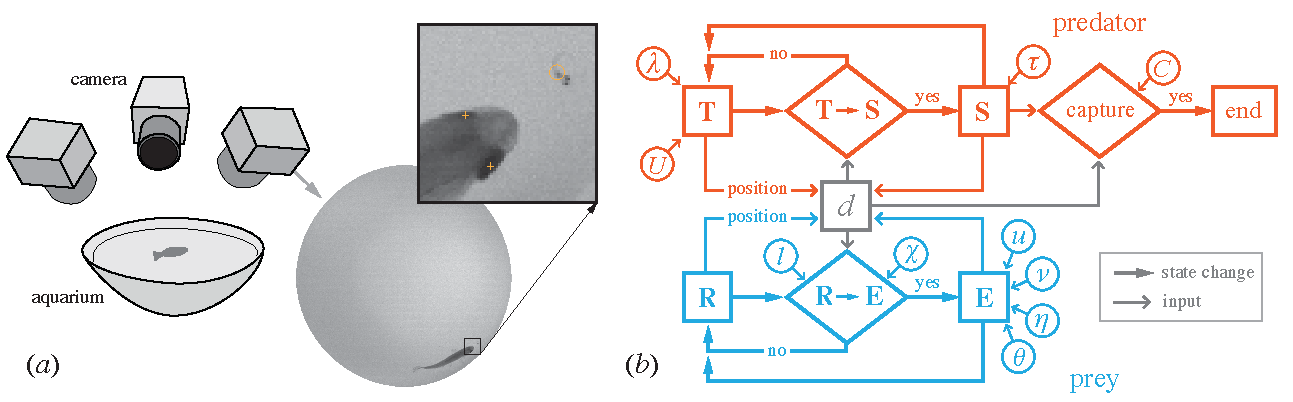
\includegraphics[width=5.5in]{fig_setup}
\caption{
Kinematic measurements and mathematical modeling for studying predator-prey interactions in zebrafish. 
(\textit{a}) Three high-speed video cameras recorded one larval prey and one predator fish (adult or juvenile) that were placed in a hemispherical aquarium. 
A representative video frame (cropped to the margin of the aquarium) shows an adult in close proximity to the prey. 
In the inset, orange markers denote the locations of morphological landmarks used to describe the position of the two fish.
This consisted of the position of the two eyes for the predator ("+") and the posterior margin of the swim bladder in the prey (open circle). 
 (\textit{b}) A state diagram illustrates the major components of the agent-based probabilistic model used to simulate the interactions between predators and prey (see Table \ref{table} for symbol definitions and parameter values). 
Each fish behaves according to an algorithm specific to a particular behavioral state and the probability of transitioning between states is determined by random-number generators with probability distributions matching our measurements (Fig \ref{fig_PDF}).
Predators (in red) operate between tracking (T) and striking (S) states and prey are either resting (R) or escaping (E).
The outcome of a strike is determined by the capture probability ($C$, Eqn. \ref{eqn_sig}). 
Simulations of this model were performed with a Monte-Carlo method to generate probability distributions of prey survival.
See Material and methods for details.
 }
\label{fig_setup}
\end{figure}

\pagebreak

\begin{figure}[!h]
\centering
	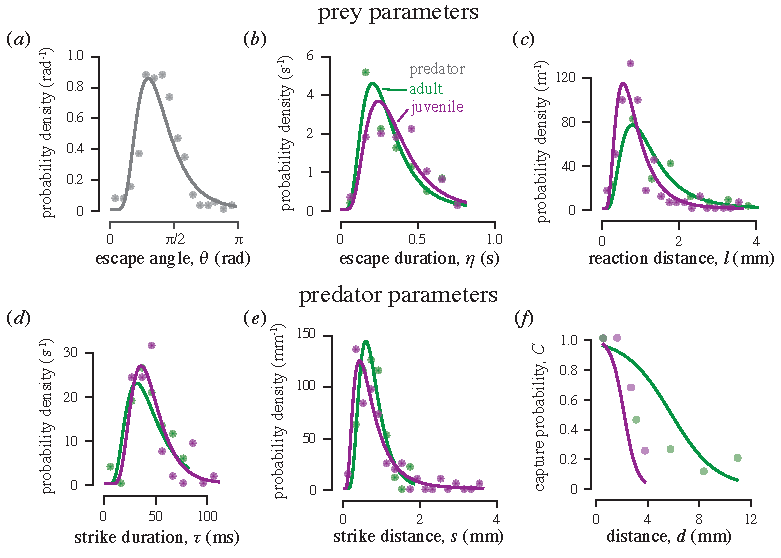
\includegraphics[width=5.5in]{fig_PDFs}
\caption{
Descriptive statistics of swimming kinematics. 
(\textit{a--e}) Measurements of the probability density (circles) for the kinematics of the prey (\textit{a--c}) and predator (\textit{d--e}) for experiments that included either a juvenile (purple) or adult (green) predator.
Points on the graphs denote measured binned values for probability density with a sample size determined using the Freedman-Diaconis rule, which yielded $N \sim 17$ measurements per point (see Table \ref{table} for total sample sizes).
Measurements of escape angle (\textit{a}) were not significantly different between the two types of experiments and these measurements were therefore combined (gray circles).
For each parameter, we performed a non-linear least-squares fit to the measurements for a log-normal probability density function (Eqn. \ref{eqn_lognorm}).
The log-mean and log-standard deviation values from these fits (Table \ref{table}) were consequently used to describe the probability of events in our mathematical model (Fig. \ref{fig_setup}\textit{b}).
(\textit{f}) The capture probability was measured as a function of distance between the predator and prey and we similarly performed a curve fit to approximate this relationship (Eqn. \ref{eqn_sig}) for our model. 
}
\label{fig_PDF}
\end{figure}

\pagebreak

\begin{figure}[!h]
\centering
	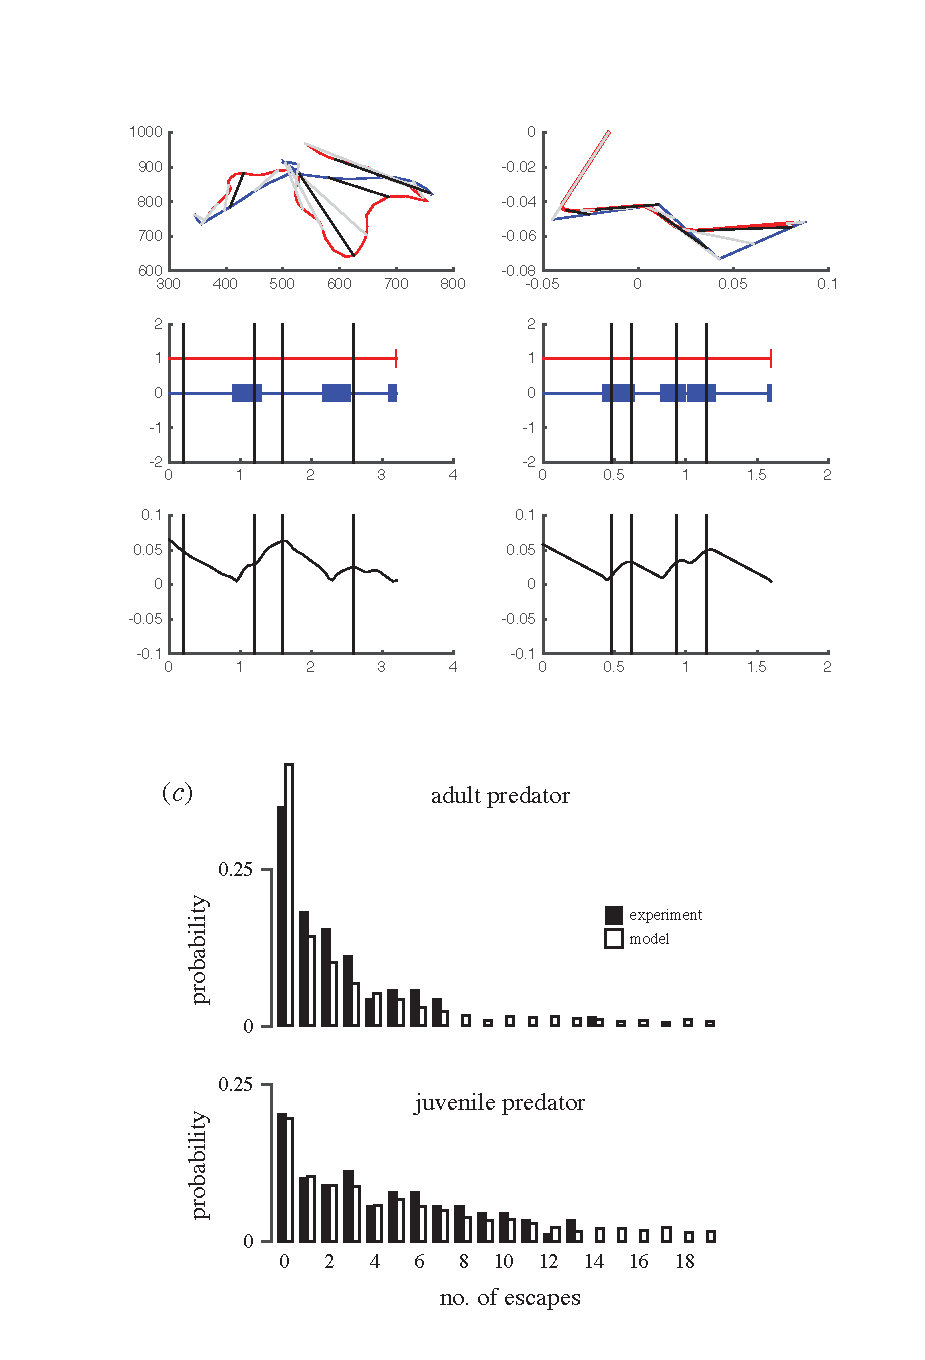
\includegraphics[width=4.5in]{fig_trajectories}
\caption{
Comparison between experimental measurements and modeling. 
(\textit{a}) Trajectories of predator and prey from a representative experiment (left) and simulation (right). 
The position of predator and prey that correspond to particular time points are shown with connecting arrows.
(\textit{b}) Ethograms for these trajectories illustrate the temporal changes in the predator's swimming and strike (left), which are respectively modeled by the tracking (T) and striking (S) (Fig. \ref{fig_setup}\textit{b}) states (right). 
The prey's behavior while motionless and during escape (left) were respectively modeled as resting (R) and escape (E) modes (right).
For both ethograms, the distance ($d$) between predator and prey are shown.
Particular moments in the trajectories are highlighted with vertical lines that correspond with the same-colored arrows in (\textit{a}).
(\textit{c}) The probability that a prey survives over a particular number of strikes is shown for adult (above) and juvenile (below) predators for experiments (dark gray) and simulations (light gray).   
}
\label{fig_traj}
\end{figure}

\begin{figure}[!h]
\centering
	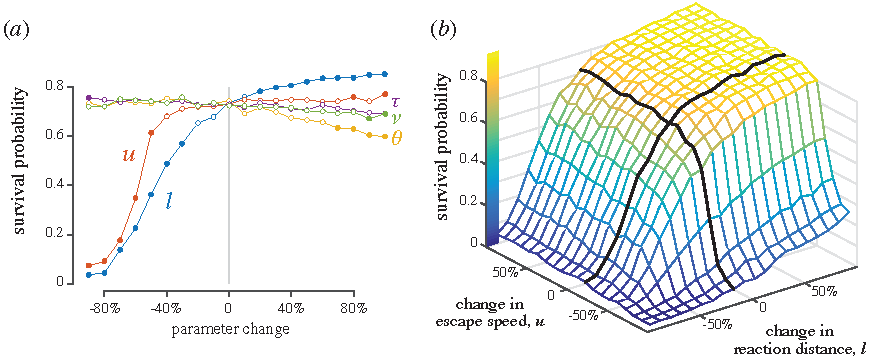
\includegraphics[width=5.5in]{fig_sensitivity}
\caption{Parameter analysis of the mathematical model to examine the effects on escape probability.  
(\textit{a}) We individually varied the mean of a parameter among simulations by manipulating the distribution (Fig. \ref{fig_PDF}) of our measurements (see Table \ref{table} for parameter definitions and values). 
Each point represents the survival probability of prey among 1000 simulations and filled circles denote a significant difference (KS-test: P < 0.05) from the observed probability.
Simulations that varied in escape angle ($\theta$) differed by a interval of 0.127 rad.
All simulations shown here used an adult predator, although similar results were obtained with a juvenile predator (Fig. S1).
}
\label{fig_sense}
\end{figure}

\pagebreak



\end{document}
